\documentclass[acmengage]{acmart}
\settopmatter{printacmref=false, printccs=false, printfolios=true}
\setcopyright{none}
\renewcommand\footnotetextcopyrightpermission[1]{}
\renewcommand{\shortauthors}{}
\renewcommand\acmBooktitle{}
\renewcommand{\abstractname}{Abstract} % specified abstract title name
\pagestyle{plain}

% numeric citation style settings
\makeatletter
\def\NAT@cmprs{\z@}
\makeatother

\usepackage{listings}
\usepackage{xcolor}
\usepackage{tcolorbox}
\usepackage{booktabs}
\usepackage{tikz}
\usetikzlibrary{arrows.meta,positioning}

\AtBeginDocument{%
  \providecommand\BibTeX{{%
    Bib\TeX}}}

\begin{document}

\fancyhead{} % Clear all headers
\fancyfoot{} % Clear all footers
\fancyfoot[C]{\thepage} % Keep page numbers centered at bottom

\title{Vector Join} % or GPU accelerated Vector Join


\author{Yayen Lin}
\email{yayen@cs.wisc.edu}
\authornote{Both authors contributed equally to this research.}
\affiliation{%
  \institution{University of Wisconsin-Madison}
  \city{Madison}
  \country{USA}
}

\author{Duke Nguyen}
\email{dnguyen56@wisc.edu}
\authornotemark[1]
\affiliation{%
  \institution{University of Wisconsin-Madison}
  \city{Madison}
  \country{USA}
}

\author{Xiangyao Yu}
\email{yxy@cs.wisc.edu}
\authornotemark[1]
\affiliation{%
  \institution{University of Wisconsin-Madison}
  \city{Madison}
  \country{USA}
}

\begin{abstract}

% in abstract we enter it with a hook
%
% and then 3 args:
%   1. OLAP remains unexplored
%   2. database engine is the perfect fit
%   3. GPU is the perfect fit
% which are then talked a bit more in detail in the introduction section

Relational data went through OLTP to OLAP decades ago: answering one row at a time and analyzing all rows at once turned out to be different problems that need different engines (use engines or solutions?). In this paper, we argue that vector search solves the OLTP half of the problem and the OLAP half remains largely unexplored and incomplete, and that GPU is the only way to scale it and database engine is the perfect fit for it. We present Sirius vector join, a prototype first class operator that integrates to and is optimized by query plan. It runs on Sirius, a GPU native SQL engine, and leverages libraries like cuVS for high-performance batched vector search (a batched vector search eventually a vector join). It achieves 165x speedup than a DuckDB vector join that uses LATERAL on the exact join path, and 227x speedup on the approximate join path using IVF-Flat index type.
\end{abstract}

\keywords{Vector Join, Vector Search, Similarity, GPU Database}

\maketitle

\section{Introduction}

% will come back and visit this section, for now just bullet points on what we wanna talk about

TBD

\section{Background}

% A bit more in detail echoing what we talked about in abstract

\begin{figure}
  \centering
  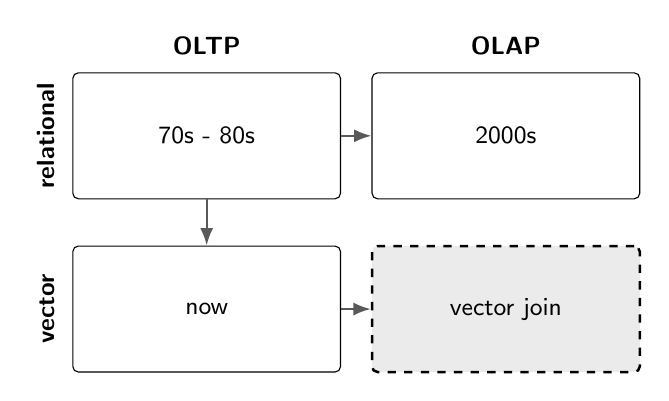
\begin{tikzpicture}[
      font=\small\sffamily,
      cell/.style={draw, rounded corners=2pt, minimum width=3.4cm,
                   minimum height=1.6cm, align=center},
      open/.style={cell, dashed, line width=0.9pt, fill=black!8},
      ax/.style={font=\small\sffamily\bfseries},
      flow/.style={-{Latex[length=2.2mm]}, thick, black!65},
    ]

    % four quadrants
    \node[cell] (a) at (0,0)      {70s - 80s};
    \node[cell] (b) at (3.8,0)    {2000s};
    \node[cell] (c) at (0,-2.2)   {now};
    \node[open] (d) at (3.8,-2.2) {vector join};

    % arrows
    \draw[flow] (a) -- (b);
    \draw[flow] (c) -- (d);
    \draw[flow] (a) -- (c);

    % column axis (x)
    \node[ax, anchor=south] at ([yshift=3pt]a.north) {OLTP};
    \node[ax, anchor=south] at ([yshift=3pt]b.north) {OLAP};

    % row axis (y)
    \node[ax, rotate=90, anchor=south] at ([xshift=-3pt]a.west) {relational};
    \node[ax, rotate=90, anchor=south] at ([xshift=-3pt]c.west) {vector};
  \end{tikzpicture}
  \caption{Relational data moved from transactional processing (OLTP,
    70s--80s) to analytical processing (OLAP, 2000s). Vector data is at
    the same inflection point: vector search answers one query at a time
    (OLTP, now), while the analytical quadrant, the vector join, is
    largely unexplored.}
  \label{fig:quadrant}
\end{figure}


In the history of database, the focus shifted from OLTP, one query, an index, an answer in milliseconds, to OLAP, where the question becomes what matches ``what'' instead of what matches ``this''. After OLTP became mature, we've seen the shift and how OLAP has become popular in many different fields that involve data analysis. We believe vector data is at the same inflection point. A vector search asks what's similar to this, when we want to ask what's similar to what, it becomes a vector join, a many-to-many instead of one-to-many (Figure~\ref{fig:quadrant}). Vector search is now a mature and crowded market, served by a number of dedicated engines~\cite{WangMilvus21, PineconeDocs, WeaviateDocs, QdrantDocs, ValdDocs} or integrated into traditional databases~\cite{PgvectorRepo, DuckDBVSS, ClickHouseVSS, SnowflakeVector, BigQueryVectorSearch, SQLServer2025Vector, MySQLHeatWaveVector}. What is missing is the other half. We see a lack of complete systems or vendors that provide vector join operations, and we believe there is going to be a similar transition of the focus, because the workloads for vector join already exist and are in great demand.

\subsection{Vector Joins and Their Applications}

% this parapgrah we can explore more use cases

A vector \emph{search} answers a point query: given one query vector, return its top-$k$ nearest neighbors from a corpus with latency as the primary concern. A vector \emph{join} answers a set query: given a table $R$ of probe vectors and a table $S$ of corpus vectors, return, for the whole of $R$, the neighbors in $S$ that satisfy a similarity condition (top k nearest or some distance threshold). The difference is the same one that separates a key lookup from a hash join.

This shape recurs across analytical workloads. In machine learning pipelines, semantic deduplication joins a training corpus against itself to find and remove near-duplicate data points; pruning this redundancy has been shown to improve both data efficiency and downstream model quality~\cite{AbbasSemDeDup23}. In data integration, entity resolution matches records across two sources by the similarity of their learned embeddings rather than by exact keys, turning a classically hard matching problem into an embedding similarity join~\cite{SantanaEMJoin25, SantanaRibeiro23}. In retrieval and recommendation, an entire batch of user or query embeddings is scored against a catalog or document corpus at once, for offline candidate generation, evaluation, or the mining of hard negatives that train the next embedding model~\cite{HuangFBRetrieval20, XiongANCE21, ThakurBEIR21}. In every case the work is inherently batched.

The demand is now surfacing in native SQL language itself. Apache Spark has a standing proposal for a \texttt{NEAREST BY} top-$k$ ranking join~\cite{ApacheSparkJIRA56395}, Databricks SQL already ships a \texttt{NEAREST BY} clause~\cite{DatabricksNearestBy26}, and recently DuckDB~\cite{DuckDBNearestByPR24137}. The declarative surface for vector joins is beginning to standardize, which sharpens the open question: how to \emph{execute} one efficiently.

\subsection{Vector Joins Are Relational Joins}

% this paragraph we can argue a little more on this topic and reflect our implementation, and we can add "for more detail refer to the implementation section" to bring readers into the implementation section

The reason the vector join belongs in a database, rather than a vector-search library, is that it is a relational join. Its join predicate is a non-equi condition that ranks candidate pairs by distance, and it is followed by a reduction that selects which ranked pairs survive: the $k$ nearest per row of $R$ (per-row top-$k$), the $k$ nearest pairs overall (global top-$k$), or every pair within a distance threshold (a radius join). These are the vector analogues of the reductions that OLAP engines already optimize, and the \texttt{NEAREST BY} proposals encode exactly this structure~\cite{ApacheSparkJIRA56395, DatabricksNearestBy26}.

Treating it as a join brings the standard toolbox to work with. Reductions can be pushed into the join so that only surviving pairs are ever materialized, in the same spirit as pushing a limit or an aggregate below a join. More importantly, the join can be \emph{partitioned}. A hash join partitions by a hash of the join key so that only co-partitioned rows are compared; a vector join partitions by \emph{semantic} proximity, clustering both sides so that a query row is compared only against corpus rows in nearby clusters. This is precisely the structure of IVF-style approximate search, recast as a partitioned join, and it is what lets one operator span the spectrum from exact (compare against everything, or against a small in-memory cluster) to approximate (probe only the nearest clusters) with the same relational machinery.

\subsection{Why the GPU}

% This section we can show more of our understanding about the type of workloads and use cases we've identified and show that GPU is the perfect fit for this kind of even-more-compute-intensive workload.

Relational OLAP is the heavier sibling of OLTP, and the intuition carries an expectation that the analytical vector workload should be heavier too. The opposite is true on modern hardware. The core of a vector join is the computation of pairwise distances between a batch of query vectors and a batch of corpus vectors, which for the common metrics reduces to a dense matrix--matrix product. This is the single operation GPUs are built to saturate, and the batched, table-sized query side of a join is what turns a memory-bound, launch-overhead-dominated single-query search into a compute-bound GEMM that keeps the tensor cores busy.

Two consequences follow. First, throughput at the scale a join demands is attainable on a single device, using the same GPU-resident vector primitives that libraries such as cuVS~\cite{NvidiaCuVS26} expose. Second, and more surprising, \emph{exact} joins become affordable across a large regime: a tiled brute-force join computes the distance matrix in blocks and never materializes it in full, so the answer is exact where CPU systems were pushed toward approximate search for cost reasons alone. Building the operator inside a GPU-native SQL engine~\cite{Yogatama26} keeps it on the device alongside the scans, filters, and aggregations of the surrounding query, so the vector join is one operator in a pipeline rather than a call out to a separate system.

\section{Motivation}
\label{sec:motivation}

% other arguments -- TBD

TBD.

\section{Technical \#1: Exact}

TBD.

\section{Technical \#2: Approximate}

TBD.

\section{Implementation}
\label{sec:implementation}

TBD.

\section{Evaluation}
\label{sec:evaluation}

TBD.

\section{Discussion}
\label{sec:discussion}

TBD.

\section{Conclusion}
\label{sec:conclusion}

TBD.

%% the bibliography file
\bibliographystyle{ACM-Reference-Format}
\bibliography{base}

\end{document}
